\chapter{Aplicações web com MEAN \textit{Stack}}	 
\label{implementacao}

%\section{Aplicação Math Race  desenvolvido com outras tecnologias}

    No capitulo três foi apresentado cada elemento do MEAN \textit{Stack} individualmente. Neste capítulo será apresentado e analisado, como estes elementos funcionam em conjunto, formando uma pilha (\textit{Stack}).

Na seção \ref{Comparativo em relação a arquitetura de aplicações LAMP} é apresentado um comparativo entre o MEAN \textit{Stack} e a arquitetura LAMP. A integração das ferramentas do MEAN \textit{Stack} é apresentada na seção \ref{Aplicação Math Race com MEAN Stack}. Na seção \ref{subsec: Testes de desempenho}  são  mostrados os testes realizados em relação ao desempenho.

A figura \ref{fig:MEAN Stack visto como uma pilha} ilustra a pilha que é formada unindo as tecnologias já explicadas no capítulo anterior. No banco de dados coloca-se o MongoDB, no lado do servidor existe o Node.js e o Express e por último no lado do cliente o AngularJS. A seta de duplo sentido representa que a passagem de dados acontece em ambos os sentidos. O principal motivo para estas tecnologias funcionarem bem em conjunto, é que todas elas têm como base a linguagem Javascript, sendo que esta característica faz parte da proposta do MEAN \textit{Stack} que é o desenvolvimento de aplicações web escaláveis com a utilização de um conjunto de ferramentas em Javascript.
    
\begin{figure}[htb]
\centering
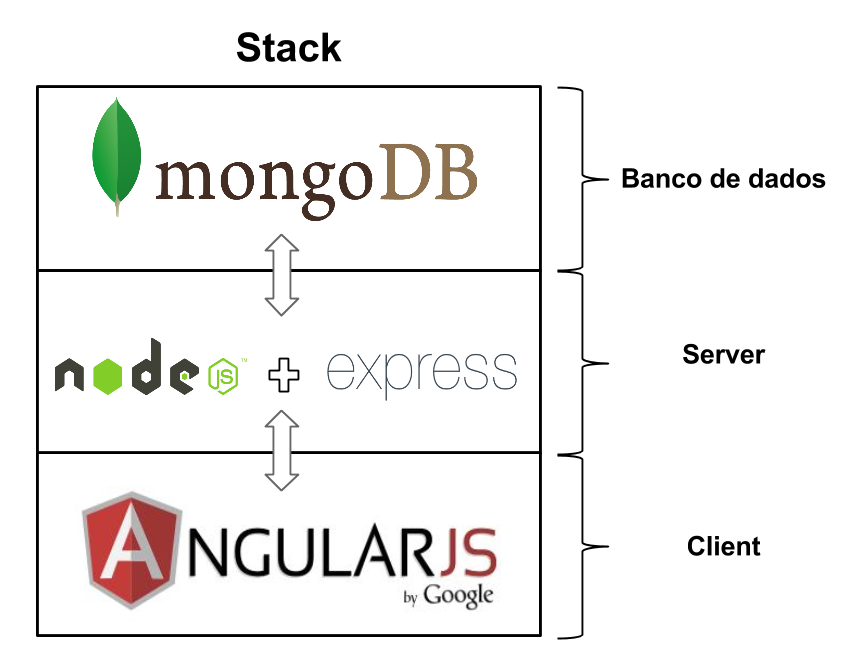
\includegraphics[scale=0.4]{images/mean_stack_diagram.png}
\caption{MEAN \textit{Stack} visto como uma pilha}
\label{fig:MEAN Stack visto como uma pilha}
\end{figure}

\newpage   
  
\section{Comparativo em relação ã arquitetura de aplicações LAMP}
\label{Comparativo em relação a arquitetura de aplicações LAMP}
    Para cada componente da pilha existe uma quantidade razoável de tecnologias semelhantes. Se for utilizada  como exemplo a figura \ref{fig:Gráfico Comparando Frameworks Javascript}, mostrada no capítulo \ref{tecnologias}, pode-se observar uma grande quantidade de tecnologias concorrentes que existem, cada uma se destacando em alguma situação. Neste cenário torna-se muito complicado concluir o que é melhor, ainda mais que o próprio MEAN pode variar, por exemplo para PEAN quando o MongoDB é substituído pelo PostgreSQL. 
    A comparação do MEAN será feita com o LAMP, pois este tem um destaque quando o assunto se trata de aplicações web. \cite{meanVSlamp}
   
   Assim como o MEAN, o LAMP é uma pilha de software livres com o foco no desenvolvimento web. A sigla LAMP é um acrônimo de Linux, Apache, MySQL e Perl/PHP/Python.
   
   Uma característica que difere os dois conjuntos de ferramentas, é que o LAMP necessita do Linux ou outro sistema operacional, ficando dependente do sistema escolhido. Enquanto o MEAN pode ser executado em qualquer plataforma.
   
    O servidor do MEAN é o Node.js, enquanto ao do LAMP é Apache. O que destaca o Node.js neste caso é o fato de ser totalmente não bloqueante e ser orientado a eventos, como já citado na subseção 3.1.4, o que permite concorrência entre as requisições. Porém como o Node.js é recente, não existe muitos \textit{plugins} que auxiliam seu uso, o que não acontece com o Apache, que já está há muito tempo no mercado, sem dizer que em muitos casos ele é escolhido como servidor padrão de muitos desenvolvedores.
    
    O Banco de dados do MEAN é o MongoDB, que como já explicado anteriormente pertence a categoria NoSQL. O LAMP utiliza o MySQL, que pertence a categoria SQL. Para comparação entre esses bancos de dados deve-se considerar a situação, por exemplo uma consulta com intuito de retornar um valor no MongoDB é mais rápida do que no MySQL, pois o MongDB não possui \textit{schemas} de tabelas mas sim um arquivo \textit{JSON}. Em contrapartida, a atualização dos dados do banco pode ser muito lenta para o MongoDB, isso considerando que existem muitos dados armazenados no banco.
    
    Para o desenvolvimento da aplicação no lado do cliente, o MEAN e o LAMP seguem abordagens consideravelmente diferentes, enquanto no MEAN \textit{Stack} a ferramenta responsável é o AngularJS, no LAMP não há uma ferramenta padrão definida.  
    
    No lado do servidor, o MEAN \textit{Stack} utiliza o  Express.js e o Node.js, e o LAMP, pode ser codificado através de três linguagens de programação: Perl, PHP ou Python.
    
    No MEAN, o Express.js serve como a camada de controle, empacotando os dados e enviando para AngularJS que utiliza a informação para realizar alguma ação e renderizar a página. A principal vantagem de se utilizar o AngularJS é que ele funciona totalmente no lado do cliente, como já foi explicado no capítulo anterior.
    
    Todas as características citadas nesta seção podem ser observadas, de forma mais direta, na tabela \ref{fig:tabela mean vs lamp}.
    
    O fato de todas as tecnologias do MEAN serem em Javascript, garante que o desenvolvedor precise saber apenas uma linguagem de programação. Porém isso também tem seu lado negativo, que é o engessamento do projeto só em Javascript, ou seja seu projeto fica dependente apenas do que o Javascript consegue fazer.
    
    % \begin{figure}[htb]
    % \centering
    % 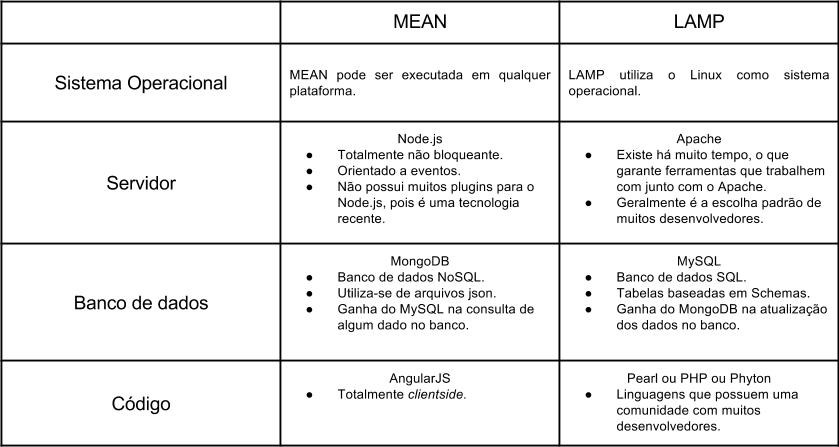
\includegraphics[scale=0.5]{images/mean_vs_lamp.png}
    % \caption{Tabela de comparação entre MEAN vs LAMP}
    % \label{fig:tabela mean vs lamp}
    % \end{figure}

\begin{table}[ht]
\centering
\begin{tabular}{|p{4cm}|p{5cm}|p{5cm}|}
\hline
\rowcolor[HTML]{CFCFCF} 
    & MEAN                                                                                                                   & LAMP                                                                                                                   \\ \hline
    Sistema Operacional & Pode ser executada em qualquer plataforma. & Utiliza o Linux como sistema operacional. \\ \hline
    Servidor 
    
    & \textbf{Node.js} 
    
    - Totalmente não bloqueante. 
    
    - Orientado a eventos. 
    
    - Não possui muitos plugins para o Node.js, pois é uma tecnologia recente. 
    
    & \textbf{Apache}
    
    - Existe há muito tempo, o que garante ferramentas que trabalhem com junto com o Apache. 
    
    - Geralmente é a escolha padrão de muitos desenvolvedores. \\ \hline
    Banco de dados & \textbf{MongoDB} 
    
    - Banco de dados NoSQL. 
    
    - Utiliza-se de arquivos JSON. 
    
    - Ganha do MySQL na operação de consulta no banco de dados. 
    
    & \textbf{MySQL} 
    
    - Banco de dados SQL. 
    
    - Tabelas baseadas em \textit{Schemas}. 
    
    - Ganha do MongoDB na atualização dos dados no banco. \\ \hline
    
    Codificação & \textbf{AngularJS}
    
    - No lado do cliente. 
   
    \textbf{Express.js} e \textbf{Node.js} 
    
    - No lado do servidor & \textbf{Pearl}, \textbf{PHP} ou \textbf{Phyton} 
    
    - No lado do servidor.  
    
    - Possuem uma comunidade com muitos desenvolvedores.  \\ \hline
\end{tabular}
\caption{Tabela de comparação entre MEAN vs LAMP}
\label{fig:tabela mean vs lamp}
\end{table}

\newpage
   
\section{Aplicação \textit{Math Race} com MEAN \textit{Stack}}
\label{Aplicação Math Race com MEAN Stack}
Nesta seção será apresentada uma aplicação desenvolvida com o MEAN \textit{Stack}. A subseção \ref{subsec: Proposta de desenvolvimento} descreve a proposta de desenvolvimento da aplicação. A subseção \ref{subsec: Utilização e funcionamento da aplicação} mostra como é a utilização e o funcionamento da aplicação. A subseção \ref{subsec: Desenvolvimento da aplicação} aborda como foi desenvolvida a aplicação. 

\subsection{Proposta da aplicação}
\label{subsec: Proposta de desenvolvimento}
 Uma aplicação simples foi desenvolvida, com o intuito de demonstrar diversos aspectos do MEAN \textit{Stack}, como a organização e a integração das ferramentas que compõem o MEAN \textit{Stack}. A aplicação foi baseada na implententação do \textit{Math Race}, desenvolvida por Iván Loire\cite{MathRace}, possuindo apenas o Node.js e o Socket.io como ferramentas em comum.

\subsection{Utilização e funcionamento da aplicação}
\label{subsec: Utilização e funcionamento da aplicação}
 A aplicação é um jogo, cujo objetivo é realizar uma competição em tempo real, para ver qual jogador acerta mais operações de matemáticas aleatórias de adição e subtração, em determinado tempo.

Na figura \ref{fig:Imagem da interface da aplicação} é mostrada a interface da aplicação, que contém a operação aleatória, o campo para entrada de dados, o marcador de tempo (\textit{Time}), o campo de pontuação (\textit{score}) e o Hall da fama (\textit{Hall of fame}).

    \begin{figure}[htb]
    \centering
    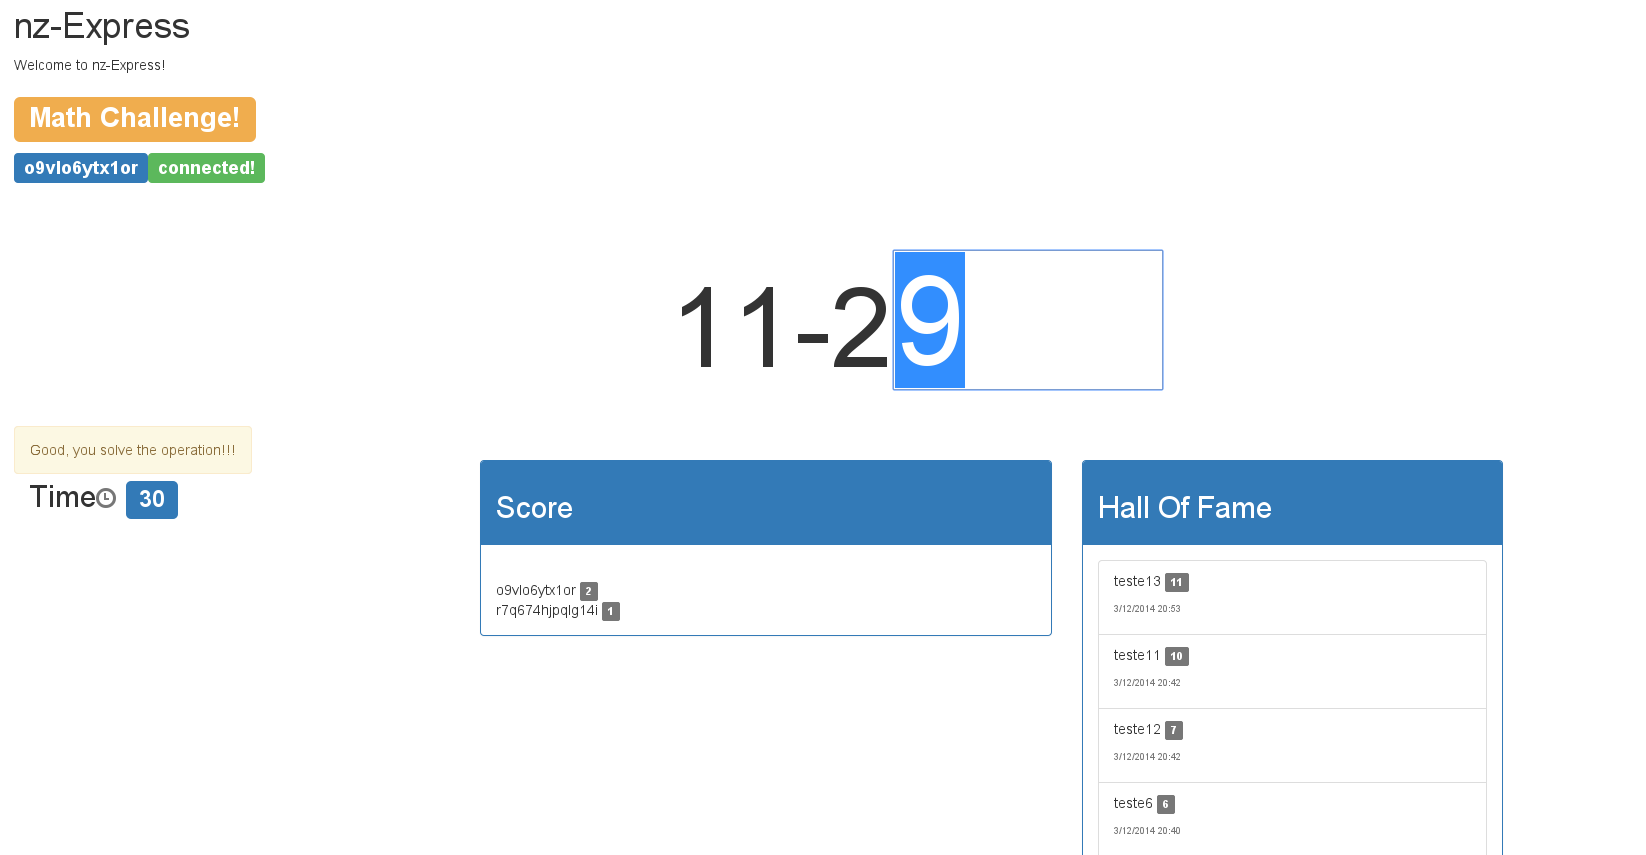
\includegraphics[scale=0.3]{images/index_mean_math_race.png}
    \caption{Imagem da interface da aplicação}
    \label{fig:Imagem da interface da aplicação}
    \end{figure}
    
Todos os jogadores possuem o mesmo tempo para responder a mesma operação matemática. A operação matemática muda para todos os jogadores após a resposta correta da operação anterior ter sido preenchida por qualquer jogador.

O jogo funciona através de rodadas, e para cada rodada o usuário tem um tempo limite pré-determinado para acertar o resultado da conta. A cada resultado correto o valor da pontuação do usuário, que começa em zero, é incrementado com mais um ponto. Ao final de uma rodada os usuários que efetuaram alguma pontuação são adicionados no ``Hall da fama'', que é ordenado pelos dez usuários com mais pontos obtidos em uma única rodada, e as pontuações dos usuários são zeradas, para que uma nova rodada se inicie. 

Na figura \ref{fig: Diagrama do funcionamento da aplicação} é demonstrado, através de um diagrama, o funcionameto da aplicação. 

    \begin{figure}[htb]
    \centering
    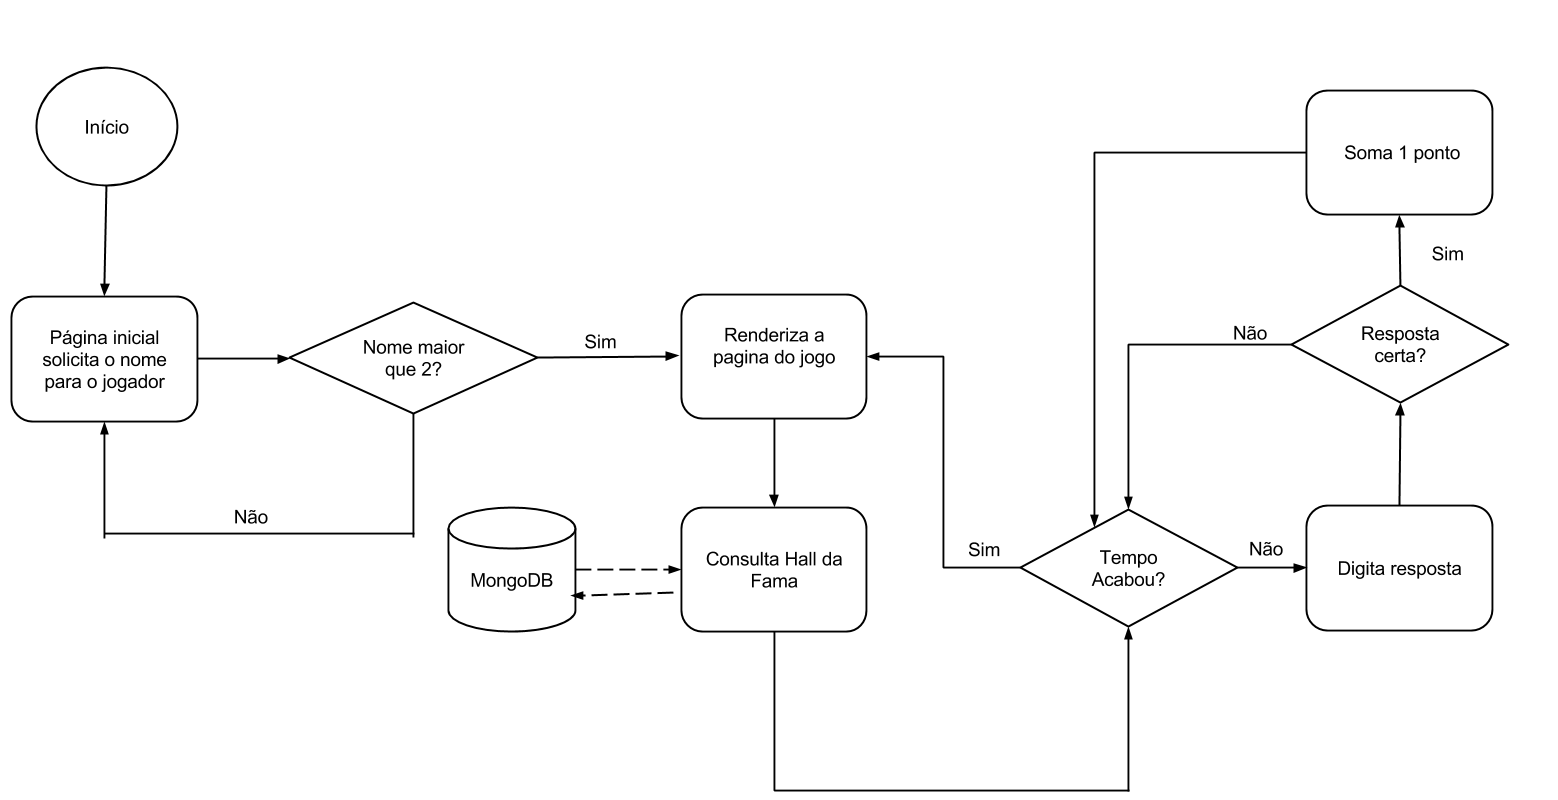
\includegraphics[scale=0.30]{images/func_mr.png}
    \caption{Diagrama do funcionamento da aplicação}
    \label{fig: Diagrama do funcionamento da aplicação}
    \end{figure}

\subsection{Desenvolvimento da aplicação}
\label{subsec: Desenvolvimento da aplicação}
Nesta subseção será abordado como é o desenvolvimento de uma aplicação baseado no MEAN \textit{Stack}. Partindo de como foi realizada a escolha da estrutura da aplicação, e finalizando com a integração das ferramentas do MEAN \textit{Stack}.
\begin{description}
\item[Estrutura da aplicação] \hfill \\
No início do desenvolvimento da aplicação, verificou-se as possibilidades em relação à estrutura e organização de arquivos que seria utilizada, pois não exite uma abordagem padrão em relação a este assunto.

Nas pesquisas iniciais as primeiras possibilidades que apareceram foram através do MEAN.js e o MEAN.io que são geradores automáticos de estruturas de arquivos para o MEAN \textit{Stack}. Apesar de fornecerem uma estrutura pronta, ao lidar com geradores, é necessário que se programe de uma maneira pré-determinada de acordo com o gerador escolhido, o que torna a aplicação um pouco mais complexa de ser apresentada, e detalhada, e foge do escopo desta monografia.

A opção escolhida para a criação da estrutura de diretórios, foi através de um submódulo do Express.js chamado \textit{express-generator}. A figura \ref{fig: estrutura criada pelo express-generator} mostra como as pastas e os arquivos são organizados neste gerador, ao total são 7 pastas e 9 arquivos. 

    \begin{figure}[htb]
    \centering
    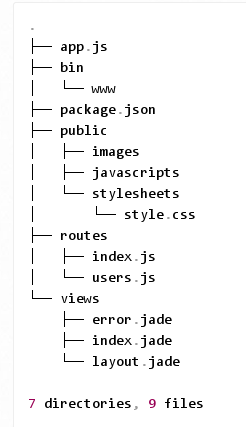
\includegraphics[scale=0.7]{images/estrutura_exp_gen.png}
    \caption{Estrutura criada pelo express-generator \cite{ExpressGen}}
    \label{fig: estrutura criada pelo express-generator}
    \end{figure}

A pasta \textit{public} contém todos os arquivos de imagem, Javascript e CSS que serão enviados para o cliente, como por exemplo os arquivos Javascript do Angular.js, e o arquivo CSS chamado style.css.

Na pasta \textit{views} são definidas as páginas da aplicação, contendo a página do \textit{layout}, do \textit{index}, e uma página de erros. Quando o usuário acessa a aplicação, primeiramente é carregada a página de \textit{layout}, que então carrega a página \textit{index}, e caso algum erro ocorra é enviada uma mensagem de erro.

Para as rotas que definem como serão tratadas as requisições que podem ser realizadas pela aplicação, o \textit{express-generator} cria uma pasta chamada \textit{routes}. Ao receber requisições, o servidor através de funções definidas na pasta \textit{routes}, pode desde renderizar as páginas solicitadas, até encaminhar as requisições para outras rotas, afim de, por exemplo, realizar uma consulta em um banco de dados.

A parte do servidor que o Node.js é responsável, fica no arquivo www da pasta \textit{bin}, e no arquivo app.js na raiz da aplicação.  

Além da estrutura criada pelo \textit{express-generator}, foram criadas mais duas pastas, que são a \textit{models} e a \textit{lib}. Na \textit{models}, ficam os arquivos responsáveis pela conexão e pelos acessos ao MongoDB. A \textit{lib} contém as principais funções da aplicação responsáveis pelo funcionamento do jogo \textit{Math Race}, e da comunicação cliente/servidor, que é feita através do Socket.io, sendo que a sua explicação foi colocada na seção \ref{sec: Socket.io} do apêndice A.

\item[Integração das ferramentas do MEAN \textit{Stack}] \hfill \\
Quando o usuário acessa a aplicação, ocorre uma série de mensagens, entre o lado do cliente e do servidor, afim de informar o servidor que há um novo usuário conectado, e fazer com que o cliente obtenha os dados da partida. 

O diagrama da figura \ref{fig: Diagrama de sequência do acesso da aplicação}, demonstra a sequência de mensagens que ocorrem quando um usuário acessa a aplicação (mensagem 1). 

No lado do servidor, o Node.js envia os arquivos da pasta \textit{public} e o \textit{index} da aplicação (mensagem 2). No lado do cliente, o Angular.js envia uma solicitação de conexão através da função \textit{connect} do Socket.io (mensagem 3), e o Node.js responde com uma mensagem avisando que o usuário está conectado (mensagem 4). Ao receber essa mensagem o Angular.js envia outra mensagem chamada ``\textit{join}'' (mensagem 5), e o Node.js envia os dados referente a operação, a pontuação e o \textit{hall} da fama (mensagem 6, 7 e 8). Por último o Angular.js faz um requisição ao MongoDB para obter o hall da fama atualizado (mensagem 9). 

    \begin{figure}[htb]
    \centering
    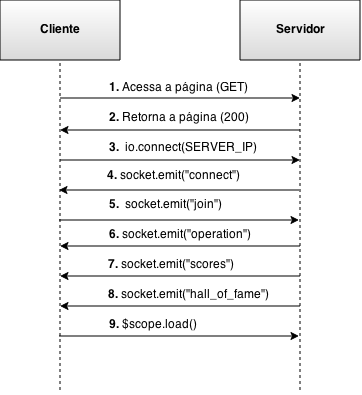
\includegraphics[scale=0.7]{images/diagrama_de_seq_acesso.png}
    \caption{Diagrama de sequência do acesso da aplicação}
    \label{fig: Diagrama de sequência do acesso da aplicação}
    \end{figure}
% codigo do join

A cada final de rodada, o Node.js envia uma nova operação, e o Angular.js envia uma mensagem ao Node.js solicitando o \textit{hall} da fama atualizado. Essa mensagem é enviada através de um módulo do Angular.js chamado \textit{ng-resource}, sendo que através deste módulo é possível interagir com o Node.js utilizando o RESTFul\footnote{ ``RESTful é um serviço web que utiliza o paradigma de arquitetura do REST, ou seja, é o termo normalmente usado para se referir a implementação de Web Services que utilizam tal arquitetura.''\cite{RESTWiki}}. 

Caso o usuário tenha efetuado alguma pontuação na rodada, o Angular.js envia uma mensagem ao Node.js, contendo um objeto JSON com o nome e a pontuação efetuada. O Node.js então faz a inserção no MongoDB, se for um novo usuário, ou atualiza a pontuação, se o nome do usuário já estiver cadastrado no MongoDB, e a nova pontuação for maior do que a antiga.

% diagrama demonstrando a aplicação em execução
\end{description}

% \begin{lstlisting}
% 	$scope.sendResult = function(item) {
% 		if (item.value) {
% 		    ...
% 			socket.emit('send-server-result', item);
% 		};
% 	}
% \end{lstlisting}

\section{Testes de desempenho}
\label{subsec: Testes de desempenho}
Nesta seção serão apresentados os testes que foram realizados através de duas aplicações, o \textit{Math Race} e o ``Encurtador de URL''. 

No \textit{Math Race}, foi efetuado um teste simples através do envio de um conjunto de requisições para consultas ao banco de dados, obtendo-se o tempo de duração para o servidor responder cada conjunto de requisições, além da média de requisições por segundo.

A aplicação ``Encurtador de URL'' foi implementada em diversos ambientes, definidos na tabela \ref{fig: Ambientes dos testes}, afim de avaliar o consumo da memória, a utilização da CPU, e a quantidade de requisições realizadas por tempo. 

\subsection{Testes na Aplicação \textit{Math Race}}
% Nesta subseção o objetivo é demonstrar o comportamento da aplicação através de um conjunto de testes de envio de requisições e consultas ao banco de dados. 
Os testes foram realizados aumentando gradativamente a quantidade de requisições e requisições concorrentes, afim de verificar a latência de resposta do servidor. A cada requisição é realizada uma consulta no banco de dados para obtenção da lista dos dez primeiros usuários e suas pontuações no \textit{hall} da fama.

Na figura \ref{fig: Lista de objetos retornada pelo MongoDB}, podemos observar parte da lista de objetos retornada pela consulta ao banco de dados, que cada cliente realiza ao acessar a aplicação durante os testes.

    \begin{figure}[htb]
    \centering
    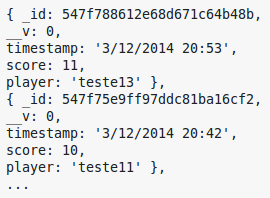
\includegraphics[scale=0.7]{images/objs_hof_bd.png}
    \caption{Lista de objetos retornada pelo MongoDB}
    \label{fig: Lista de objetos retornada pelo MongoDB}
    \end{figure}
% \begin{lstlisting}
% \end{lstlisting}

A máquina utilizada nos testes tem como configurações um Core i7 de 3.6GHZ, e 8GB de memória RAM, utilizando o Fedora 20 de 64 \textit{bits} como sistema operacional.


Na tabela \ref{fig: Carga na quantidade requisições} são mostrados os resultados dos testes realizados na aplicação, através de uma ferramenta específica para teste de carga (\textit{Load test}) conhecida como \textit{weighttp}\footnote{http://redmine.lighttpd.net/projects/weighttp/wiki}. No \textit{weighttp} é possível definir parâmetros como a quantidade de requisições que serão enviadas ao servidor e o número de requisições concorrentes que ocorrerão durante o teste.

Para estes testes foram imaginados dois cenários diferentes, sendo determinada uma quantidade de requisições concorrentes fixa (100 e 1000) em cada cenário. Para cada cenário variou-se a quantidade de requisições de 1.000 até 100.000, obtendo-se o tempo demorado pelo servidor para atender todas estas requisições e a taxa de requisições por segundo. 


\begin{table}[ht]
\centering
\begin{tabular}{|c|c|c|c|}
\hline
\rowcolor[HTML]{CFCFCF} 
\# requisições concorrentes & \# requisições & tempo(seg) & req/seg      \\ \hline
\rowcolor[HTML]{EFEFEF} 
\cellcolor[HTML]{EFEFEF} & 1000 & 0,69 & 1458  \\ \cline{2-4}
\rowcolor[HTML]{EFEFEF} 
\cellcolor[HTML]{EFEFEF} & 2000 & 1,357 & 1472  \\ \cline{2-4}
\rowcolor[HTML]{EFEFEF} 
\cellcolor[HTML]{EFEFEF} & 5000           & 3,437      & 1454  \\ \cline{2-4} 
\rowcolor[HTML]{EFEFEF} 
\cellcolor[HTML]{EFEFEF} & 10000          & 7,690      & 1414  \\ \cline{2-4} 
\rowcolor[HTML]{EFEFEF} 
\cellcolor[HTML]{EFEFEF} & 30000          & 20,928     & 1433  \\ \cline{2-4} 
\rowcolor[HTML]{EFEFEF} 
\cellcolor[HTML]{EFEFEF} & 50000          & 34,986     & 1429  \\ \cline{2-4} 
\rowcolor[HTML]{EFEFEF} 
\cellcolor[HTML]{EFEFEF} & 70000          & 47,102     & 1486  \\ \cline{2-4} 
\rowcolor[HTML]{EFEFEF}
\multirow{-8}{*}{\cellcolor[HTML]{EFEFEF}100} & 100000 & 67,967     & 1471  \\ \hline
    & 1000           & 3,250      & 330   \\ \cline{2-4} 
    & 2000           & 3,350      & 658   \\ \cline{2-4} 
    & 5000           & 3,691      & 1354  \\ \cline{2-4} 
    & 10000          & 7,503      & 1332  \\ \cline{2-4} 
    & 30000          & 21,963     & 1365  \\ \cline{2-4} 
    & 50000          & 37,327     & 1339  \\ \cline{2-4} 
    & 70000          & 52,157     & 1342  \\ \cline{2-4} 
\multirow{-8}{*}{1000}   & 100000         & 74,914     & 1334  \\ \hline    
\end{tabular}
\caption{Carga na quantidade requisições}
\label{fig: Carga na quantidade requisições}
\end{table}

Pode-se notar através da tabela \ref{fig: Carga na quantidade requisições}, que à medida que carga de requisições aumenta, o tempo  total para o servidor responder estas requisições cresce consideravelmente, independentemente do número de requisições concorrentes, mas mantém, em média, a mesma taxa de requisições por segundo. No gráfico da figura \ref{fig: Gráfico de requisições por tempo}, pode-se visualizar de maneira mais clara o comportamento da aplicação, durante a carga de requisições.  
% \newpage
    \begin{figure}[htb]
    \centering
    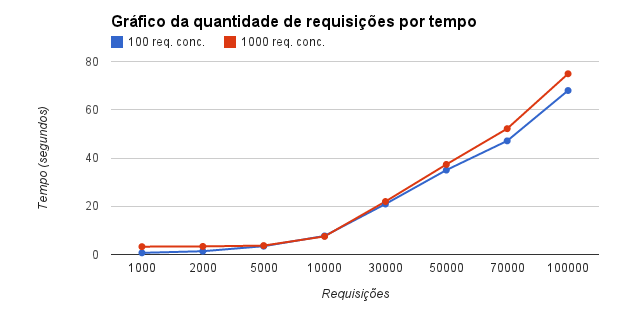
\includegraphics[scale=0.7]{images/reqxtempo.png}
    \caption{Gráfico de requisições por tempo}
    \label{fig: Gráfico de requisições por tempo}
    \end{figure}

\newpage

\subsection{Análise de testes de desempenho do Node.js e do MongoDB com outros ambientes}
Os principais componentes responsáveis pela a escalabilidade no MEAN \textit{Stack} são o MongoDB, através do \textit{autosharding}, e do mapeamento dos dados em memória, e o NodeJS, através do \textit{Event Loop}, e da \textit{Thread Pool}, como mencionado no capítulo \ref{tecnologias}.
    
Existem diversas referências que comparam o desempenho destes dois componentes juntos com outros ambientes, variando desde a linguagem de programação até a base de dados utilizada.

A referência que esta monografia irá utilizar como base é a do artigo de Ricardo Schroeder e Fernando dos Santos,  intitulado ``Arquitetura e testes de serviços web de alto desempenho com Node.js e Mongodb'' \cite{NodejsEMongodb} que implementou um ``Encurtador de URL'' como aplicação.

A aplicação do ``Encurtador de URL'' serve para mapear uma \textit{hash}, de 6 caracteres, para uma URL. Cada \textit{hash} é gerada de maneira única, e aleatória, e foram alocados um milhão de URL's para os testes.

A cada acesso é feita a verificação se a \textit{hash} utilizada é válida.  Primeiro é verificado se a \textit{hash} tem 6 caracteres e depois se ela existe no banco de dados, caso alguma destas verificações falhe é retornado somente um código de  resposta de erro 404. 

Para os testes, a aplicação definida foi implementada em 6 ambientes, que foram descritos na tabela \ref{fig: Ambientes dos testes}. Cada aplicação de um ambiente efetua a mesma requisição e será testada utilizando uma base de amostras contendo duas mil \textit{hashs}. A duração foi estipulada em 60 segundos, sendo que nos  5 segundos iniciais, foram criados quarenta usuários que irão se conectar de maneira incremental, permanecendo ativos durantes os próximos quarenta e cinco segundos e reduzindo durante os dez segundos finais. 

\begin{table}[htb]
\centering
\begin{tabular}{|c|c|c|}
\cline{1-3}
\rowcolor[HTML]{CFCFCF}
Servidor & Linguagem de Programação & Banco de Dados \\ \cline{1-3}
Node.JS  & Javascript               & MongoDB        \\ \cline{1-3}
Node.Js  & Javascript               & PostgresSQL    \\ \cline{1-3}
Netty    & Java                     & MongoDB        \\ \cline{1-3}
Netty    & Java                     & PostgresSQL    \\ \cline{1-3}
Apache   & PHP                      & MongoDB        \\ \cline{1-3}
Apache   & PHP                      & PostgresSQL    \\ \cline{1-3}
\end{tabular}
\caption{Ambientes dos testes \cite{NodejsEMongodb}}
\label{fig: Ambientes dos testes}
\end{table}

Os testes realizados na aplicação foram executados em um ambiente virtualizado contendo as seguintes características: Sistema Operacional CentOS 6.2 x86, 1Gb de memória RAM, 2 núcleos de 2,4Ghz Intel Core I5. A aplicação utilizada para os testes foi o JMeter, que é um software que serve para realizar testes de desempenho, carga e stress, desenvolvido pela Apache\footnote{http://jmeter.apache.org/} . Os resultados são mostrados nas tabelas \ref{fig:graf_memoria}, \ref{fig:graf_cpu} e \ref{fig:graf_tempo}.
\clearpage
\begin{description}
\item[Consumo de Memória RAM] \hfill \\
A memória RAM é um dos princípais pontos de análise em um servidor web, pois está ligada diretamente ao número de requisições que o servidor é capaz de atender em determinado tempo.\cite{NodejsEMongodb}
O resultado do teste demonstrou o uso de memória constante e estabilidade por parte de cada plataforma. Os piores resultados ficaram com os ambientes que utilizam o servidor Apache e a linguagem PHP, enquanto o ambiente que usa Node.js e o MongoDB foi o segundo melhor no índice de consumo de memória.

\begin{figure}[htb!]
\centering
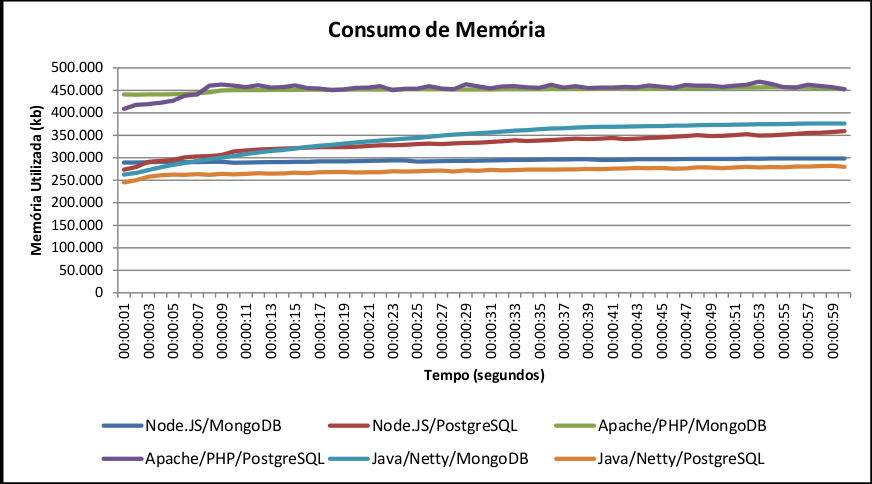
\includegraphics[scale=0.5]{images/graf_memoria.png}
\caption{Consumo de memória RAM durante a execução dos testes \cite{NodejsEMongodb}}
\label{fig:graf_memoria}
\end{figure}

\clearpage
 
\item[Utilização de CPU] \hfill \\
Analisar a utilização de CPU é um fator relevante para que se tenha uma noção da carga gerada pelas requisições efetuadas pelos clientes. Quanto mais próximo de 100\% estiver o uso da CPU, maiores serão as chances do servidor não conseguir atender as requisições recebidas. 

No gráfico da figura \ref{fig:graf_cpu} nota-se um melhor desempenho do Node.js junto ao MongoDB em relação aos outros ambientes, ficando com 40\% de uma média de uso, enquanto em outros ambientes como o que utilizou Java/Netty/PostgreSQL este consumo passou para aproximadamente 90\%.

\begin{figure}[htb]
\centering
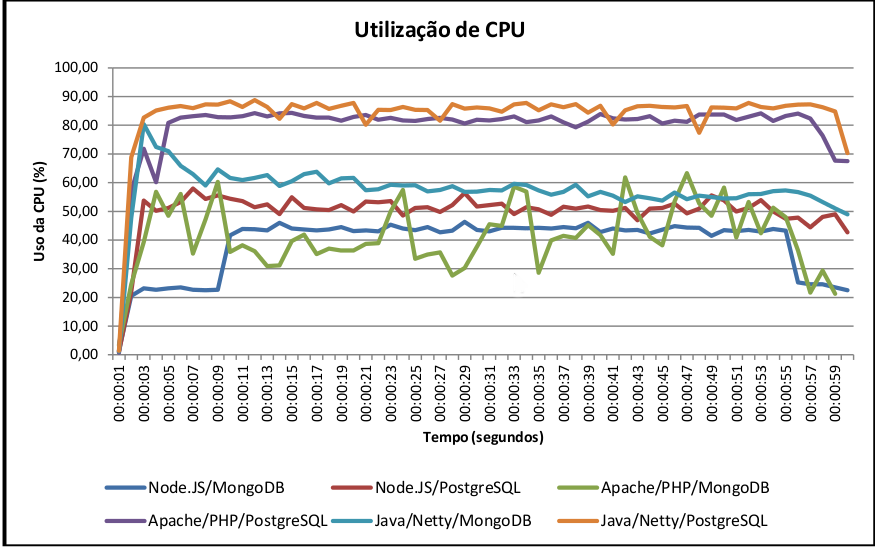
\includegraphics[scale=0.5]{images/graf_cpu.png}
\caption{Consumo de CPU (\%) durante a execução do teste. \cite{NodejsEMongodb}}
\label{fig:graf_cpu}
\end{figure}

% \newpag
\clearpage
\item[Quantidade de requisições por tempo] \hfill \\
O teste de requisições por tempo basicamente indica o quanto de usuários (requisições) o servidor é capaz de absorver.\cite{NodejsEMongodb}

Na figura \ref{fig:graf_tempo} é possível observar que os dois ambientes que mais responderam requisições, que no caso foram o Node.JS/MongoDB e o Netty/MongoDB, utilizaram o mesmo banco de dados. Mas o crédito desse resultado positivo, também se deve aos servidores de alto desempenho, que possuem como característica atender o maior numero de requisições simultâneas. Outro ponto que chama atenção, é como os ambientes com MongoDB se destacaram sobre os ambientes com PostgresSQL.

% \clearpage
\begin{figure}[htb]
% \centering
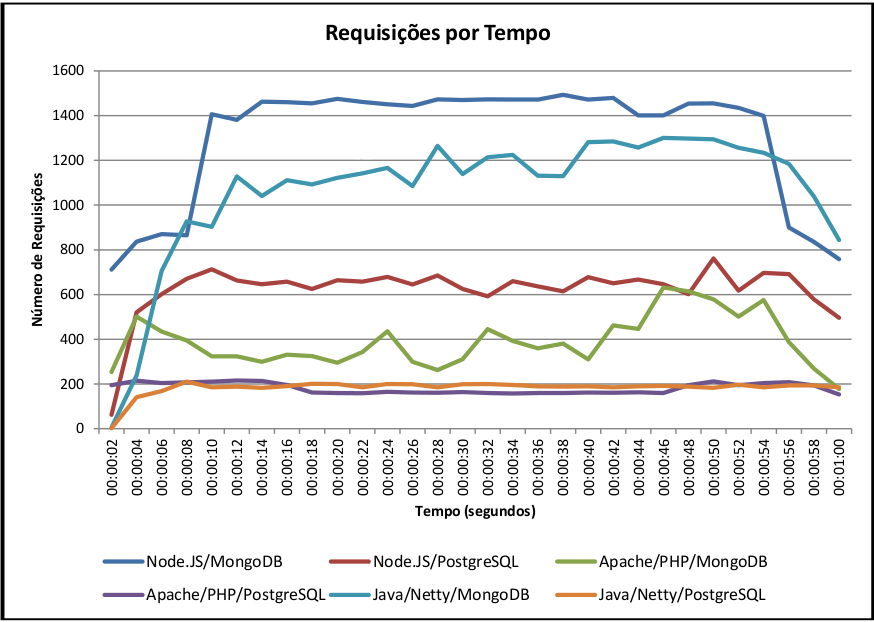
\includegraphics[scale=0.5]{images/graf_req_tempo.png}
\caption{Requisições por tempo. \cite{NodejsEMongodb}}
\label{fig:graf_tempo}
\end{figure}

\end{description}


Após ser realizada uma análise dos testes, tanto no \textit{Math Race} quanto no ``Encurtador de URL'', concluímos que realmente a utilização do Node.js junto ao MongoDB, proporciona um ganho de desempenho considerável, em relação as tecnologias comparadas. Este ganho se deve ao fato das particularidades que cada tecnologia adota, para lidar com escalabilidade, no caso o Node.js com o \textit{Event Loop} e o MongoDb com o \textit{Autosharding}.
%de maneira pura, ou seja, sem que haja alteração para obtenção de resultados  



% PROPOSTA DE DESENVOLVIMENTO

% DIAGRAMA DE CASOS DE USO
%  Especificações dos cs

% DESENVOLVIMENTO DA APLICAÇÃO

% UTILIZAÇÃO DA APLICAÇÃO

%  TESTES DE DESEMPENHO
%   weigthttp
%   objetivo do teste, como foram realizados, hardware utilizado
%      analise dos resultados obtidos

%   figura

% analise dos teste

